\documentclass[reqno, 12pt]{amsart}
\usepackage[utf8]{inputenc}
\usepackage{amsfonts}
\usepackage{mathtools}
\usepackage{amsthm,amssymb}
\usepackage{graphicx} 
\usepackage{enumitem}
\usepackage{tikz}
\usepackage{hyperref}
\usepackage[section]{placeins}
\usepackage[percent]{overpic}
\usetikzlibrary{spath3, intersections, hobby, knots, arrows.meta, backgrounds}
\usepackage{pgfplots}
\usepgfplotslibrary{fillbetween}
\pgfplotsset{compat=1.18}
\usepackage{float}
\usepackage{verbatim}

	\oddsidemargin =0.0in
	\evensidemargin=0.0in
	\textwidth=6.5in
	\headheight=0.0in
	\topmargin=0.0in
	\textheight=8.5in

\theoremstyle{remark}
\newtheorem{claim}{Claim}
\newtheorem*{claim*}{Claim} 
\newtheorem{theorem}{Theorem}
\newtheorem{definition}{Definition}
\newtheorem*{remark*}{Remark}

\newenvironment{subproof}[1][\proofname]{%
\renewcommand{\qedsymbol}{$\blacksquare$}%
\begin{proof}[#1]%
}{%
\end{proof}%
}

\title{\resizebox{\textwidth}{!}{\textbf{COMPUTING THE KNOT FLOER HOMOLOGY OF $(1,1)$-KNOTS}}}
\author{CLAYTON JORDAN}
\date{}

\pagestyle{plain}

\begin{document}

\maketitle

\section{Introduction}
\subsection{Knots}
What is a knot? Knots are easy to define; a knot $K$ is a smooth embedding of $S^1$ into $\mathbb{R}^3$, also known as a smooth, closed loop that lives in $3$-dimensional space. We consider knots equivalent up to ambient isotopy. The trivial knot is called  the unknot; it is the knot with no twists or tangles.
\begin{figure}[H]
	\centering
		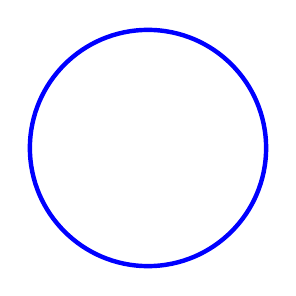
\begin{tikzpicture}
			\draw[ultra thick,blue] (0,0) circle[radius=1.5cm];
		\end{tikzpicture}
	\caption{A diagram of the unknot in $\mathbb{R}^2$.}
\end{figure}
The foundational problem in knot theory is: given two knot diagrams $K_1$ and $K_2$, how can we tell if $K_1$ and $K_2$ represent the same knot, or different knots?

\subsection{Reidemeister Moves and Knot Invariants}
How can we tell if two diagrams describe the same knot? One way is to check if we can transform one diagram into the other via a sequence of \textit{Reidemeister moves}. Reidemeister moves are local moves, meaning they only affect a small part of the knot diagram.
\begin{figure}[H]
	\centering
		\includegraphics[width=0.4\textwidth]{reidemeister.png}
		\caption{The three types of Reidemeister moves.}
	\label{fig:reidemeister}
\end{figure}
Kurt Reidemester proved in 1927 that two diagrams belong to the same knot if and only if one can be transformed into the other through an appropriate sequence of these three moves (\textit{Reidemeister's Theorem}).
\begin{figure}[H]
	\centering
	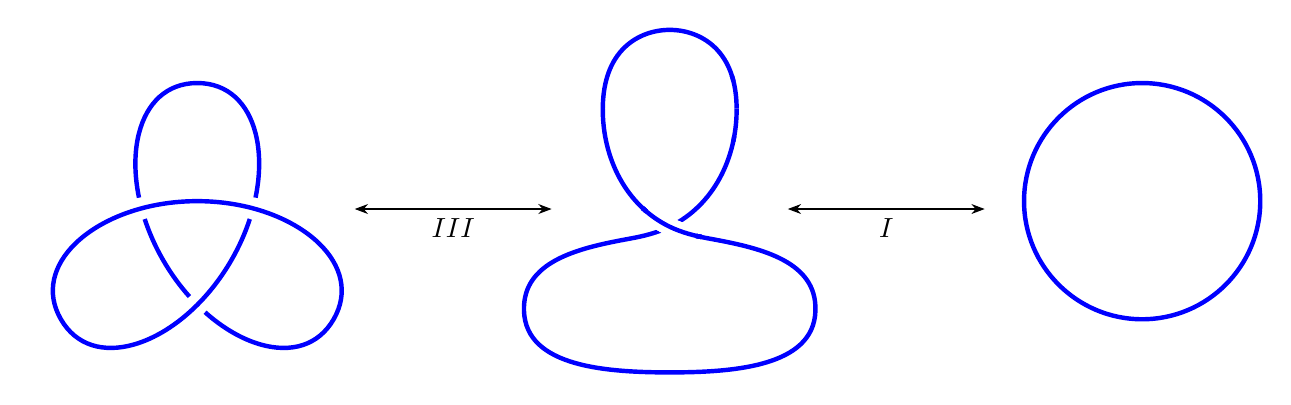
\begin{tikzpicture}[
		use Hobby shortcut,  
		every trefoil component/.style={ultra thick, draw, blue},
		]
		\begin{scope}[shift={(0,0)}]
			\path[spath/save=trefoil] ([closed]90:2) foreach \k in {1,...,3} { .. (-30+\k*240:.5) .. (90+\k*240:2) } (90:2);
			\tikzset{spath/knot={trefoil}{8pt}{0,1,5}}
		\end{scope}
		\draw [Stealth-Stealth] (2,0.4) -- (4.5,0.4) node[below, midway] {$III$};
		\begin{scope}[shift = {(5,-0.325)}]
			\begin{knot}[
				consider self intersections=true,
				ignore endpoint intersections=false,
				clip width=4,
				flip crossing=1,
				]
				\strand[ultra thick, blue]
				([closed]1.85,2) .. (1.6, 2.75) .. (1,3) .. (0.4,2.75) .. (0.15,2) .. (1,0.5) .. (1.5,0.35) .. (2.85,-0.5) .. (1,-1.35).. (-0.85,-0.5) .. (0.5,0.35) .. (1,0.5) .. (1.85,2);
			\end{knot}
		\end{scope}
		\draw [Stealth-Stealth] (7.5,0.4) -- (10,0.4) node[below, midway] {$I$};
		\begin{scope}[shift={(12,0.5)}]
			\draw[ultra thick,blue] (0,0) circle[radius=1.5cm];
		\end{scope}
	\end{tikzpicture}
	\caption{We can see that these are both diagrams for the unknot by applying a type $III$ Reidemeister move, followed by a type $I$ Reidemeister move, or vice-versa.}
	\label{fig:fig3}
\end{figure}
These moves are important when defining \textit{knot invariants}. 	A \textit{knot invariant} is a property $\phi$ defined on the set of all knot diagrams such that given a knot $K$, for any two diagrams $D_1, D_2$ of $K$ we have $\phi(D_1)=\phi(D_2)$. If we can define a property on the set of knot diagrams, then show that for any arbitrary knot diagram, the property assigned to that diagram is not affected by Reidemeister moves, then we have defined a knot invariant. Various knot invariants are used to help distinguish knots, or to determine that two knot diagrams actually represent the same knot. They vary in type from integers, to polynomials, to algebraic structures. The simplest of these invariants is a Boolean invariant called \textit{tricolorability}; we say a knot $K$ is \textit{tricolorable} if given any diagram for $K$, we can colour the strands in the diagram in a manner such that:
	\begin{enumerate}[nosep]
		\item All three colours are used to colour the diagram.
		\item At each crossing in the diagram, the meeting strands must be all different colours, or all the same colour.
	\end{enumerate}
	Tricolorability is infact an invariant: one proves this by showing that for a knot diagram $K_1$, if $K_1$ is tricolorable, then any knot diagram obtained by performing one Reidemeister move on $K_1$ is still tricolorable, and if $K_1$ is not tricolorable, then any knot diagram obtained by performing one Reidemeister move on $K_1$ is still not tricolorable.
\begin{figure}[htb!]
	\centering
		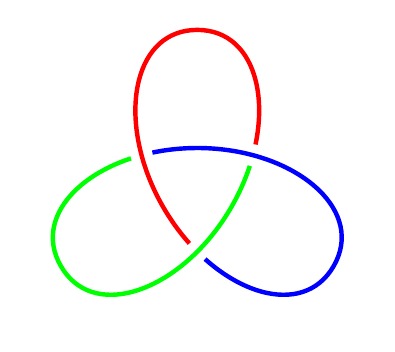
\begin{tikzpicture}[
			use Hobby shortcut,
			every trefoil component/.style={ultra thick, draw, red},
			trefoil component 1/.style={blue},
			trefoil component 2/.style={green},
			]
			\path[spath/save=trefoil] ([closed]90:2) foreach \k in {1,...,3} { .. (-30+\k*240:.5) .. (90+\k*240:2) } (90:2);
			\tikzset{spath/knot={trefoil}{8pt}{1,3,5}}
		\end{tikzpicture}
	\caption{An example of a tricolorable knot. This knot is known as the \textit{trefoil}.}
	\label{fig:fig4}
\end{figure}

\begin{figure}[H]
	\centering
		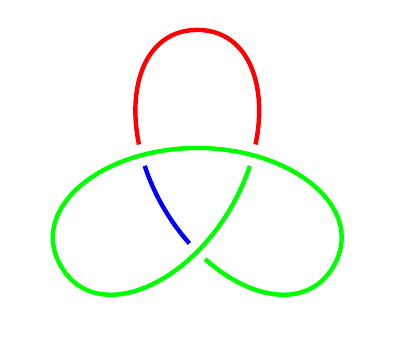
\begin{tikzpicture}[
			use Hobby shortcut,  
			every trefoil component/.style={ultra thick, draw, red},
			trefoil component 1/.style={blue},
			trefoil component 2/.style={green},
			]
			\path[spath/save=trefoil] ([closed]90:2) foreach \k in {1,...,3} { .. (-30+\k*240:.5) .. (90+\k*240:2) } (90:2);
			\tikzset{spath/knot={trefoil}{8pt}{0,1,5}}
		\end{tikzpicture}
	\caption{This knot is not tricolorable. }
\end{figure}

As seen in Figure \ref{fig:fig3}, the above is a diagram of the unknot. Hence, we see that the unknot is \textit{not} tricolorable, whereas the trefoil is tricolorable (Figure \ref{fig:fig4}). Clearly, this means that the unknot and the trefoil are \textit{not} the same knot.  We now see that there is more than one knot, and that knot theory is in fact interesting!

Tricolorability is an example of a Boolean invariant, the simplest type of invariant. The invariant we will examine in this paper is an algebraic invariant, which is much richer and more complex. The reader should note that there are many invariants of intermediate complexity, notably integer valued or polynomial valued invariants.

\subsection{Algebraic Preliminaries}
We briefly and informaly introduce some algebraic notions which are essential to knot Floer homology:
	\begin {definition}
	A \textit{chain complex}  $\mathcal{C}$ is a sequence of abelian groups $C_0, C_1, ... ,C_i$ and boundary operators $\partial_n \colon C_n \to C_{n-1}$ such that  $\partial_n \circ \partial_{n+1} \equiv 0$.
	\end{definition}
	Note the second condition implies that $\operatorname{im}(\partial_{n+1}) \subset \ker(\partial_{n})$.
	\begin {definition}
	The \textit{$n_{th}$ homology}  $\mathcal{H}$ of a chain complex is defined as $\mathcal{H}_n(\mathcal{C}) = \ker(\partial_{n}) / \operatorname{im}(\partial_{n+1})$.
	\end{definition}
	\begin {definition}
		An \textit{integer filtration} $A$ is a value assigned to a generator $x$ such that $A(\partial(x)) \le A(x)$. An \textit{integer grading} $M$ is similar, except that it satisfies $M(\partial(x)) = M(x)-1.$
	\end{definition}
	We will see specific examples of these filtrations and gradings and how they are calculated later.
	\begin{figure}[H]
		\begin{tikzpicture}[scale=1]
			\begin{axis}[
				axis lines = middle, gray!80,
				xmin=-1, xmax=4,
				ymin=-1, ymax=4,
				grid = both,
				grid style = {dashed, gray!30},
				xticklabel=\empty,
				yticklabel=\empty,
				major tick style = {transparent},
				xtick distance = 1,
				ytick distance = 1
				]
				\addplot[only marks, mark=*, black, mark size=1.4] coordinates {
				(1,3)
				(2,3)
				(2,1)
				(1,1)
				};
				\addplot[->, -{Stealth}, black, thick] coordinates {(1.8, 3) (1.2, 3)};
				\addplot[->, -{Stealth}, black, thick] coordinates {(2, 2.8) (2, 1.2)};
				\addplot[->, -{Stealth}, black, thick] coordinates {(1.8, 1) (1.2, 1)};
				\addplot[->, -{Stealth}, black, thick] coordinates {(1, 2.8) (1, 1.2)};
			\end{axis}
		\end{tikzpicture}
		\hspace{1cm}
		\begin{tikzpicture}[scale=1]
			\begin{axis}[
				axis lines = middle, gray!80,
				xmin=-1, xmax=4,
				ymin=-1, ymax=4,
				grid = both,
				grid style = {dashed, gray!30},
				xticklabel=\empty,
				yticklabel=\empty,
				major tick style = {transparent},
				xtick distance = 1,
				ytick distance = 1
				]
				\addplot[only marks, mark=*, black, mark size=1.6] coordinates {
				(1,3)
				(2,3)
				(2,1)
				(1,1)
				};
				\addplot[->, -{Stealth}, black, thick] coordinates {(1.8, 3) (1.2, 3)};
				\addplot[->, -{Stealth}, black, thick] coordinates {(2, 2.8) (2, 1.2)};
				\addplot[->, -{Stealth}, black, thick] coordinates {(1.8, 1) (1.2, 1)};
			\end{axis}
		\end{tikzpicture}
		\caption{Two operators: over $\mathbb{F}_2$, the left represents a chain complex, and the right does not.}
	\end{figure}

\section{Knot Floer Homology}
\subsection{A (very brief) Overview}
Knot Floer homology is an algebraic knot invariant discovered in 2002 by Ozsv\'ath and Szab\'o; and independently by Rasmussen in 2003. While giving a full description of this invariant is well beyond the scope of this paper, the interested reader is encouraged to read \cite{OzsvathSzabo2017} for a complete overview of the subject. It is much more complete than classical invariants like tricolorability, meaning it better distinguishes different knots. We can also extract many other invariants from its structure, making it worthwhile to compute. In the context of this paper, we are mostly interested in how we can compute it. Computing the Knot Floer homology, or $\text{HFK}^{\infty}(K)$, for a knot involves counting all holomorphic disks in its Heegaard splitting, then constructing the doubly filtered chain complex $\text{CFK}^{\infty}(K)$. Finally, we compute homology of the \textit{associated graded object} of $\text{CFK}^{\infty}(K)$. In our context, we are more interested in the chain complex $\text{CFK}^{\infty}(K)$ itself, as we can extract many interesting invariants from its structure. The main obstruction to constructing $\text{CFK}^{\infty}(K)$ is the counting of holomorphic disks, which is hard and not algorithmically viable for most knots.
\begin{figure}[H]
	\centering
		\begin{overpic}[width=0.6\textwidth]{heegaardunknot.pdf}      
			\put(44.7, 10.15){\circle*{1.5}}
			\put(49.5, 49.6){$\beta$}
			\put(40.2, 13.9){$\alpha$}
		\end{overpic}
	\caption{A Heegaard diagram for the unknot.}
\end{figure}

\subsection{Properties of $\text{CFK}^{\infty}$}
	$\text{CFK}^{\infty}(K)$ is an $\mathbb{F}[U, U^{-1}]$ module which is finitely generated by the intersection points between $\alpha$ and $\beta$ in the chosen Heegaard diagram. Each intersection point has an integer valued \textit{Alexander filtration} and \textit{Maslov grading} associated to it, which are calculated from the disks in the Heegaard diagram as we will see later. The second filtration is the \textit{$i$ filtration}: an element $U^kx$ has $i$ filtration $-k$. The formal variable $U$ acts as a diagonal shift and respects both filtrations and grading, as it strictly lowers them. $\partial$ is constructed directly from the diagram's disks. The two most important properties to note are:
\begin{enumerate}[nosep]
	\item{The boundary operator satisfies $\partial^2 \equiv 0$,  so $\text{CFK}^{\infty}(K)$ is indeed a chain complex.}
	\item{$\partial$ never raises the Alexander or $i$ filtration and strictly lowers the Maslov grading by $1$.}
\end{enumerate}
In other words, $\text{CFK}^{\infty}(K)$ is a doubly filtered, integer graded chain complex, as desired.

\subsection{The $(1,1)$ Context.}
Let $K \subset S^3$ be a knot. We say $K$ is a $(g, b)$-knot, $g, b \in \mathbb{Z}_+$, if there is a genus $g$ Heegaard splitting $V_1 \cup V_2$ of $S^3$ such that $K$ intersects $V_i$ in exactly $b$ disjoint, trivial arcs. For our purposes, it is only important to understand that any $(1,1)$-knot can be represented by a torus with two smooth, closed, embedded curves and two basepoints on its surface. 
\begin{remark*} 
The above is an extremely simplified description of $(1,1)$-knots. Those who are interested are encouraged to read \cite[Section~2.3]{Marian2020} for a much more thorough definition of this family of knots.
\end{remark*}
\begin{figure}[H]
	\centering
	\begin{overpic}[width=0.6\textwidth]{heegaardlt.pdf}
		\put(48, 12.5){\small $z$}
		\put(39.2, 5.9){\small $w$}        
		\put(47, 13.2){\circle*{1.3}}
		\put(43, 6.6){\circle{1.3}}        

		\put(45.6, 3.9){\circle*{1}}
		\put(44.5, 10.2){\circle*{1}}
		\put(45.1, 16.7){\circle*{1}}

		\put(45.8, 4.4){\tiny $3$}
		\put(44.9, 8.4){\tiny $2$}
		\put(45.6, 16.9){\tiny $1$}

		\put(49.5, 51){$\beta$}
		\put(54.3, 11.7){$\alpha$}
			
	\end{overpic}
	\caption{A doubly pointed Heegaard diagram for the trefoil, a $(1,1)$-knot.}
	\label{fig:fig5}
\end{figure}
Working in this context resolves our earlier obstruction, as holomorphic disks in these Heegaard splittings reduce to embedded disks, or bigons bounded by $\alpha$ and $\beta$, on the surface of the torus.
\begin{figure}[H]
	\centering
		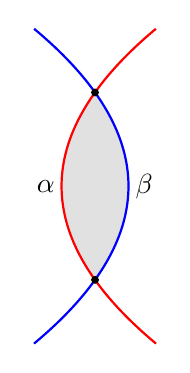
\begin{tikzpicture}
			\fill[gray!30, opacity=0.8] 
			plot[domain=-1.190:1.190, samples=100, smooth, variable=\y] ({0.3*\y*\y}, {\y}) -- 
			plot[domain=1.190:-1.190, samples=100, smooth, variable=\y] ({-0.3*\y*\y+0.85}, {\y}) -- cycle;
			\draw[domain=-2:2, samples=100, smooth, variable=\y, red, thick, name path = A]
			plot ({0.3*\y*\y}, {\y});
			\draw[domain=-2:2, samples=100, smooth, variable=\y, blue, thick, name path = B]
			plot ({-0.3*\y*\y+0.85}, {\y});
			\draw[fill=black](0.425, 1.190) circle(1.2pt);
			\draw[fill=black](0.425, -1.190) circle(1.2pt);
			\node at (-0.2, 0) {$\alpha$};
			\node at (1.05, 0) {$\beta$};
		\end{tikzpicture}
	\caption{An example of a bigon bounded by $\alpha$ and $\beta$.}
\end{figure}
Counting these disks is easy, in the sense that it can be implemented algorithmically and solved in polynomial time. By cutting along $\alpha$ and the surface of the torus aobve the last arc enclosing the $z$ basepoint, we can move to the fundamental domain of the torus in $\mathbb{R}^2$. Note that the two red sides and the two black sides of the fundamental domain are identified with each other to reconstruct the torus. Finally, we can parametrize these diagrams with a $4$-tuple $(p, a, b, r)$, where $p$ is the number of intersection points between $\alpha$ and $\beta$, $a$ is the number of rainbow arcs on each side of the diagram, $b$ is the number of arcs from below the rainbow arcs on the left to above the rainbow arcs on the right, where the first such arc connects to the $r_{th}$ point on the right side of the fundamental region. Note that each rainbow arc forms a bigon; we call these \textit{trivial disks}, and each diagram has exactly $2a$ trivial disks. We have now greatly simplified the object we are working with, as we have moved from a surface in $\mathbb{R}^3$ to a 4-tuple of positive integers which encodes the same information.
\begin{figure}[H]
	\centering
		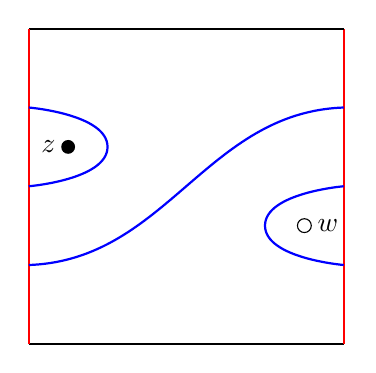
\begin{tikzpicture}[scale=1]
			\draw[thick, black] (0,0) -- (4, 0);
			\draw[thick, red] (4, 0) -- (4, 4);
			\draw[thick, black] (4, 4) -- (0, 4);
			\draw[thick, red] (0, 4) -- (0, 0);
			
			\draw[blue, thick] plot[smooth, tension=1.5]
			coordinates {(0,3) (1,2.5) (0,2)};
			
			\draw[blue, thick] plot[smooth, tension=1.5]
			coordinates {(4,2) (3,1.5) (4,1)};
			
			\draw[blue, thick] (0,1) to[out=2, in=-178] (4,3);
			
			\fill[black] (0.5,2.5) circle (2.5pt);
			\draw[black] (3.5,1.5) circle (2.5pt);
			\node at (0.25, 2.5) {$z$};
			\node at (3.8, 1.5) {$w$};
		\end{tikzpicture}
	\caption{The 4-tuple diagram $(3, 1, 1, 1)$ is obtained from the above process applied to the Heegaard diagram in Figure \ref{fig:fig5}.  Hence, $(3, 1, 1, 1)$ parametrizes the left trefoil. }
\end{figure}

\subsection{Finding the Disks}
We first establish some terminology: label all intersection points on the left of the fundamental region $1,2,...,p$ from top to bottom, and on the right, $p+1,p+2,...,2p$, with the understanding that $p+n$ and $n$ are the same intersection point. Closed areas bounded by $\alpha$ and $\beta$  are called \textit{regions}. A \textit{small region} is a region that lives in one copy of the fundamental domain. Regions are described by their \textit{gaps}, where a gap is a connected segment of $\alpha$ and is described by two intersection points $u, v$, where $u$ is the topmost intersection point of the gap, and $v$ is the bottommost. Disks are regions which have exactly one gap. To find these disks, we first find all \textit{simple} small regions and all trivial disks. 
\begin{figure}[H]
	\centering
		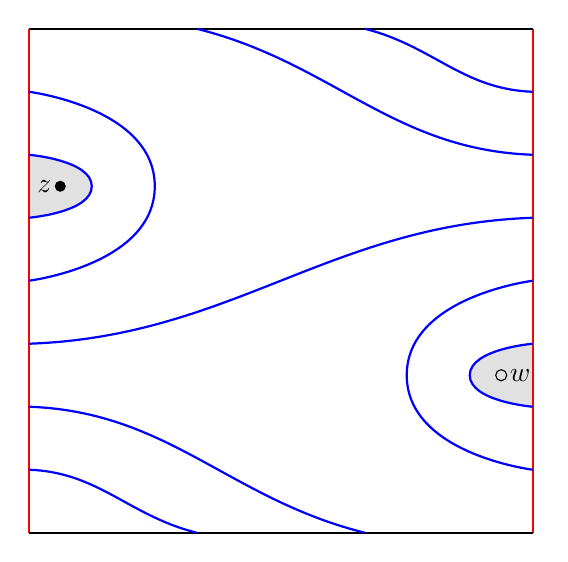
\begin{tikzpicture}[scale = 0.8]
			\draw[thick, red, name path = R, save path = \pathR] (8, 0) -- (8, 8);
			\draw[thick, black] (8, 8) -- (0, 8);
			\draw[thick, red, name path = L, save path = \pathL] (0, 8) -- (0, 0);
			\draw[thick, black] (0, 0) -- (8, 0);
			
			\draw[blue, thick] plot[smooth, tension=1.5]
			coordinates {(0,7) (2,5.5) (0,4)};
			\draw[blue, thick, name path = Ld, save path = \pathLd] plot[smooth, tension=1.5]
			coordinates {(0,6) (1,5.5) (0,5)};
			
			\draw[blue, thick] plot[smooth, tension=1.5]
			coordinates {(8,4) (6,2.5) (8,1)};
			\draw[blue, thick, name path = Rd, save path = \pathRd] plot[smooth, tension=1.5]
			coordinates {(8,3) (7,2.5) (8,2)};
			
			\draw[blue, thick] (0,3) to[out=2, in=-178] (8,5);
			
			\draw[blue, thick] (0,2) to[out=-2, in=166] (5.33333,0);
			\draw[blue, thick] (8,7) to[out=178, in=-14] (5.33333,8);
			\draw[blue, thick] (0,1) to[out=-2, in=166] (2.66667,0);
			\draw[blue, thick] (8,6) to[out=178, in=-14] (2.66667,8);

			\begin{scope}[on background layer]
				\tikzfillbetween[of=L and Ld] {gray!30, opacity=0.8};
				\tikzfillbetween[of=R and Rd] {gray!30, opacity=0.8};
			\end{scope}

			\fill[black] (0.5,5.5) circle (2.5pt);
			\draw[black] (7.5,2.5) circle (2.5pt);
			\node at (0.25, 5.5) {$z$};
			\node at (7.8, 2.5) {$w$};
		\end{tikzpicture}
		\hspace{1cm}
		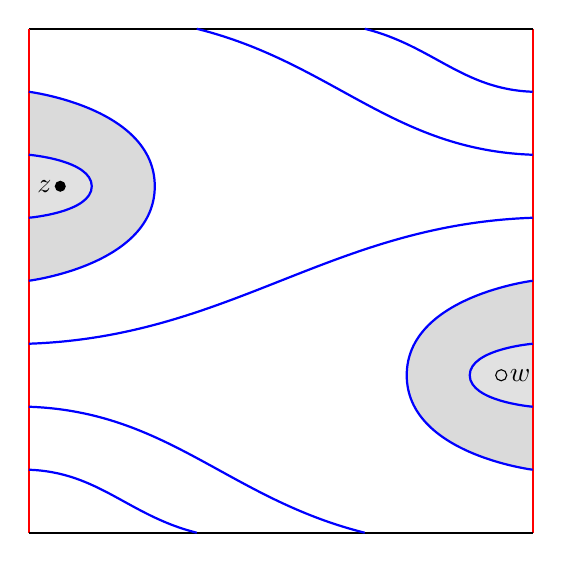
\begin{tikzpicture}[scale = 0.8]
			\draw[thick, red, name path = R, save path = \pathR] (8, 0) -- (8, 8);
			\draw[thick, black] (8, 8) -- (0, 8);
			\draw[thick, red, name path = L, save path = \pathL] (0, 8) -- (0, 0);
			\draw[thick, black] (0, 0) -- (8, 0);

			\draw[blue, thick, name path = Ld, save path = \pathLd] plot[smooth, tension=1.5]
			coordinates {(0,7) (2,5.5) (0,4)};
			\draw[blue, thick, name path = Ld1, save path = \pathLd1] plot[smooth, tension=1.5]
			coordinates {(0,6) (1,5.5) (0,5)};
			
			\draw[blue, thick, name path = Rd, save path = \pathRd] plot[smooth, tension=1.5]
			coordinates {(8,4) (6,2.5) (8,1)};
			\draw[blue, thick, name path = Rd1, save path = \pathRd1] plot[smooth, tension=1.5]
			coordinates {(8,3) (7,2.5) (8,2)};
			
			\draw[blue, thick] (0,3) to[out=2, in=-178] (8,5);
			
			\draw[blue, thick] (0,2) to[out=-2, in=166] (5.33333,0);
			\draw[blue, thick] (8,7) to[out=178, in=-14] (5.33333,8);
			\draw[blue, thick] (0,1) to[out=-2, in=166] (2.66667,0);
			\draw[blue, thick] (8,6) to[out=178, in=-14] (2.66667,8);

			\begin{scope}[on background layer]
				\tikzfillbetween[of=Ld1 and Ld] {gray!30, opacity=0.8};
				\tikzfillbetween[of=Rd1 and Rd] {gray!30, opacity=0.8};
				\tikzfillbetween[of=L and Ld] {gray!30, opacity=0.8};
				\tikzfillbetween[of=R and Rd] {gray!30, opacity=0.8};
			\end{scope}

			\fill[black] (0.5,5.5) circle (2.5pt);
			\draw[black] (7.5,2.5) circle (2.5pt);
			\node at (0.25, 5.5) {$z$};
			\node at (7.8, 2.5) {$w$};
		\end{tikzpicture}
	\caption{The four trivial disks in the 4-tuple diagram $(7, 2, 1, 3)$, shaded in grey.}
\end{figure}
A simple small region is a region bounded by two arcs which cross the diagram. 
	\begin{figure}[H]
		\centering
		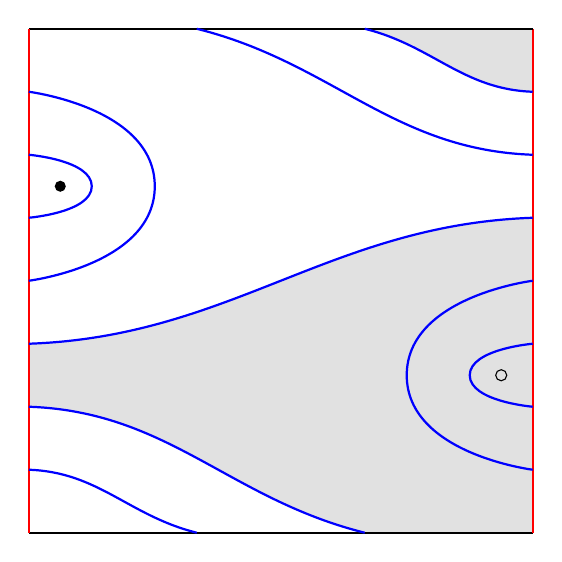
\begin{tikzpicture}[scale = 0.8]
			\draw[thick, black, name path = B] (0,0) -- (8, 0);
			\draw[thick, red] (8, 0) -- (8, 8);
			\draw[thick, black, name path = Tb] (8, 8) -- (0, 8);
			\draw[thick, red] (0, 8) -- (0, 0);
			
			\draw[blue, thick] plot[smooth, tension=1.5]
			coordinates {(0,7) (2,5.5) (0,4)};
			\draw[blue, thick] plot[smooth, tension=1.5]
			coordinates {(0,6) (1,5.5) (0,5)};
			
			\draw[blue, thick] plot[smooth, tension=1.5]
			coordinates {(8,4) (6,2.5) (8,1)};
			\draw[blue, thick] plot[smooth, tension=1.5]
			coordinates {(8,3) (7,2.5) (8,2)};
			
			\draw[blue, thick, name path = T2] (0,3) to[out=2, in=-178] (8,5);
			
			\draw[blue, thick, name path = T3] (0,2) to[out=-2, in=166] (5.33333,0);
			\draw[blue, thick, name path = T] (8,7) to[out=178, in=-14] (5.33333,8);
			\draw[blue, thick] (0,1) to[out=-2, in=166] (2.66667,0);
			\draw[blue, thick] (8,6) to[out=178, in=-14] (2.66667,8);
			
			\fill[black] (0.5,5.5) circle (2.5pt);
			\draw[black] (7.5,2.5) circle (2.5pt);
			\begin{scope}[on background layer]
				\tikzfillbetween[of=T and Tb] {gray!30, opacity=0.8};
				\tikzfillbetween[of=T2 and B] {gray!30, opacity=0.8};
				\tikzfillbetween[of=T3 and B] {white!6};
			\end{scope}
		\end{tikzpicture}
		\hspace{1cm}
		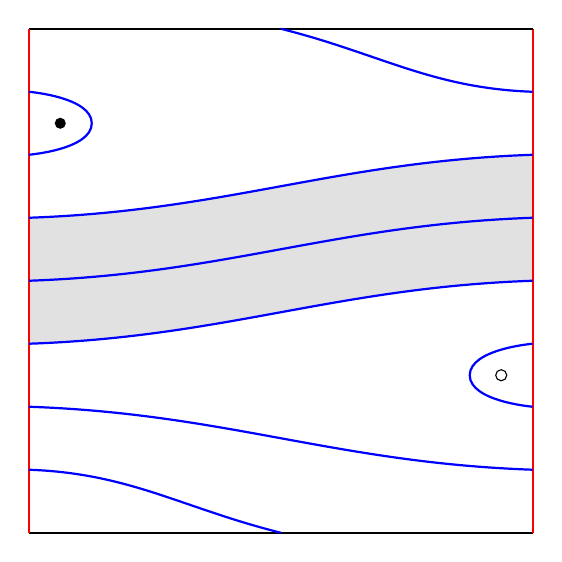
\begin{tikzpicture}[scale = 0.8]
			\draw[thick, black] (0,0) -- (8, 0);
			\draw[thick, red] (8, 0) -- (8, 8);
			\draw[thick, black] (8, 8) -- (0, 8);
			\draw[thick, red] (0, 8) -- (0, 0);
			
			\draw[blue, thick] plot[smooth, tension=1.5]
			coordinates {(0,7) (1,6.5) (0,6)};
			
			\draw[blue, thick] plot[smooth, tension=1.5]
			coordinates {(8,3) (7,2.5) (8,2)};
			
			\draw[blue, thick, name path = T] (0,5) to[out=2, in=-178] (8,6);
			\draw[blue, thick] (0,4) to[out=2, in=-178] (8,5);
			\draw[blue, thick, name path = B] (0,3) to[out=2, in=-178] (8,4);
			\draw[blue, thick] (0,2) to[out=-2, in=178] (8,1);
			
			\draw[blue, thick] (0,1) to[out=-2, in=166] (4,0);
			\draw[blue, thick] (8,7) to[out=178, in=-14] (4,8);
			
			\fill[black] (0.5,6.5) circle (2.5pt);
			\draw[black] (7.5,2.5) circle (2.5pt);
			\begin{scope}[on background layer]
				\tikzfillbetween[of=T and B] {gray!30, opacity=0.8};
			\end{scope}
		\end{tikzpicture}
		\caption{Two simple small regions in different 4-tuple diagrams.}
	\end{figure}
From this list, we form more regions by checking for each region if we can "cut out" any trivial disks that are contained in the region. It can be shown that this process will give us a complete list of small regions. 
	\begin{figure}[H]
		\centering
		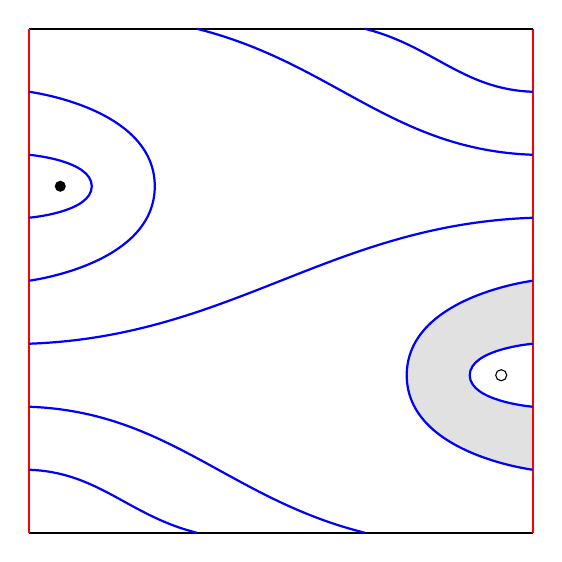
\begin{tikzpicture}[scale = 0.8]
			\draw[thick, black] (0,0) -- (8, 0);
			\draw[thick, red, name path = L] (8, 0) -- (8, 8);
			\draw[thick, black] (8, 8) -- (0, 8);
			\draw[thick, red] (0, 8) -- (0, 0);
			
			\draw[blue, thick] plot[smooth, tension=1.5]
			coordinates {(0,7) (2,5.5) (0,4)};
			\draw[blue, thick] plot[smooth, tension=1.5]
			coordinates {(0,6) (1,5.5) (0,5)};
			
			\draw[blue, thick, name path = D1] plot[smooth, tension=1.5]
			coordinates {(8,4) (6,2.5) (8,1)};
			\draw[blue, thick, name path = D2] plot[smooth, tension=1.5]
			coordinates {(8,3) (7,2.5) (8,2)};
			
			\draw[blue, thick] (0,3) to[out=2, in=-178] (8,5);
			
			\draw[blue, thick] (0,2) to[out=-2, in=166] (5.33333,0);
			\draw[blue, thick] (8,7) to[out=178, in=-14] (5.33333,8);
			\draw[blue, thick] (0,1) to[out=-2, in=166] (2.66667,0);
			\draw[blue, thick] (8,6) to[out=178, in=-14] (2.66667,8);
			
			\fill[black] (0.5,5.5) circle (2.5pt);
			\draw[black] (7.5,2.5) circle (2.5pt);
			\begin{scope}[on background layer]
				\tikzfillbetween[of=D1 and D2] {gray!30, opacity=0.8};
				\tikzfillbetween[of=D2 and L] {white!6};
			\end{scope}
		\end{tikzpicture}
		\hspace{1cm}
		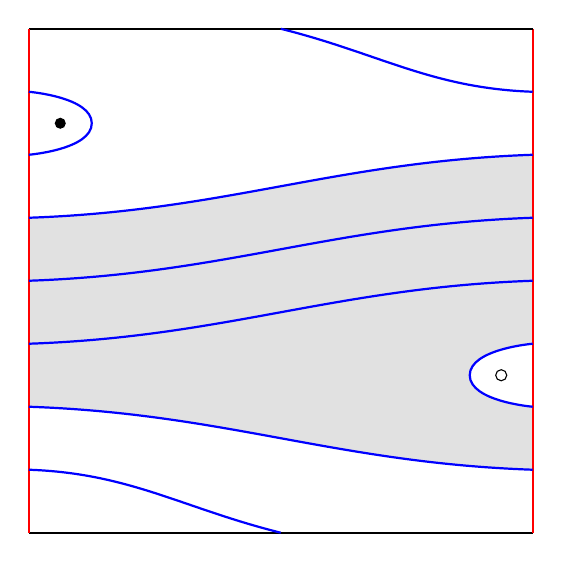
\begin{tikzpicture}[scale = 0.8]
			\draw[thick, black] (0,0) -- (8, 0);
			\draw[thick, red, name path = L] (8, 0) -- (8, 8);
			\draw[thick, black] (8, 8) -- (0, 8);
			\draw[thick, red] (0, 8) -- (0, 0);
			
			\draw[blue, thick] plot[smooth, tension=1.5]
			coordinates {(0,7) (1,6.5) (0,6)};
			
			\draw[blue, thick, name path = D] plot[smooth, tension=1.5]
			coordinates {(8,3) (7,2.5) (8,2)};
			
			\draw[blue, thick, name path = T] (0,5) to[out=2, in=-178] (8,6);
			\draw[blue, thick] (0,4) to[out=2, in=-178] (8,5);
			\draw[blue, thick] (0,3) to[out=2, in=-178] (8,4);
			\draw[blue, thick, name path = B] (0,2) to[out=-2, in=178] (8,1);
			
			\draw[blue, thick] (0,1) to[out=-2, in=166] (4,0);
			\draw[blue, thick] (8,7) to[out=178, in=-14] (4,8);
			
			\fill[black] (0.5,6.5) circle (2.5pt);
			\draw[black] (7.5,2.5) circle (2.5pt);
			\begin{scope}[on background layer]
				\tikzfillbetween[of=T and B] {gray!30, opacity=0.8};
				\tikzfillbetween[of=D and L] {white!6};
			\end{scope}
		\end{tikzpicture}
		\caption{Two cut out small regions.}
	\end{figure}
Now, for each small region, we check if we can attach a disk to all but one of the region's gaps. If we can, we add a new disk to our list, determined exactly by the gap that we didn't attach a disk to. We repeat this process until we run through all regions without adding a new disk. 
\newsavebox{\mypicboxone}
	\savebox{\mypicboxone}{
		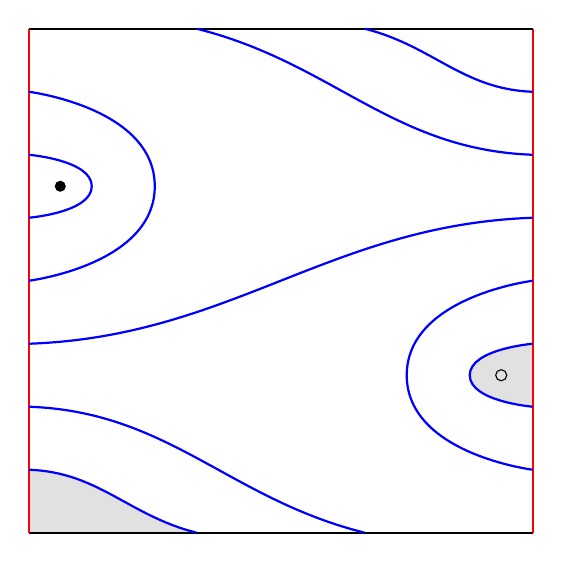
\begin{tikzpicture}[scale=0.8]
			\draw[thick, black, name path = B] (0,0) -- (8, 0);
			\draw[thick, red, name path = L] (8, 0) -- (8, 8);
			\draw[thick, black] (8, 8) -- (0, 8);
			\draw[thick, red] (0, 8) -- (0, 0);
			
			\draw[blue, thick] plot[smooth, tension=1.5]
			coordinates {(0,7) (2,5.5) (0,4)};
			\draw[blue, thick] plot[smooth, tension=1.5]
			coordinates {(0,6) (1,5.5) (0,5)};
			
			\draw[blue, thick] plot[smooth, tension=1.5]
			coordinates {(8,4) (6,2.5) (8,1)};
			\draw[blue, thick, name path = D] plot[smooth, tension=1.5]
			coordinates {(8,3) (7,2.5) (8,2)};
			
			\draw[blue, thick] (0,3) to[out=2, in=-178] (8,5);
			
			\draw[blue, thick] (0,2) to[out=-2, in=166] (5.33333,0);
			\draw[blue, thick] (8,7) to[out=178, in=-14] (5.33333,8);
			\draw[blue, thick, name path = T] (0,1) to[out=-2, in=166] (2.66667,0);
			\draw[blue, thick] (8,6) to[out=178, in=-14] (2.66667,8);
			
			\fill[black] (0.5,5.5) circle (2.5pt);
			\draw[black] (7.5,2.5) circle (2.5pt);
			\begin{scope}[on background layer]
				\tikzfillbetween[of=T and B] {gray!30, opacity=0.8};
				\tikzfillbetween[of=D and L] {gray!30, opacity=0.8};
			\end{scope}
		\end{tikzpicture}
	}
\newsavebox{\mypicboxtwo}
	\savebox{\mypicboxtwo}{
		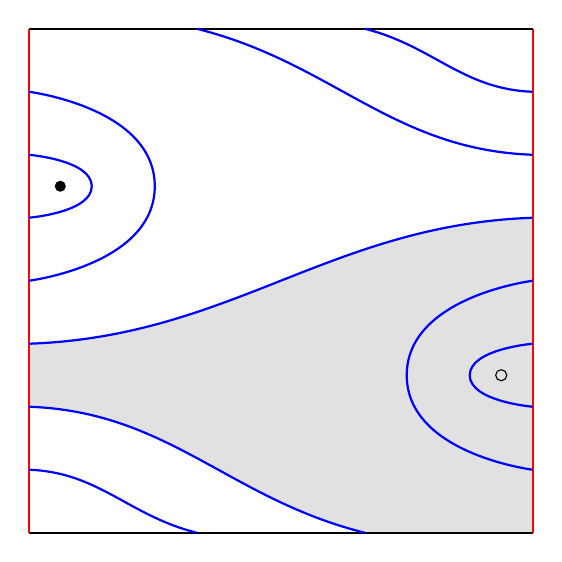
\begin{tikzpicture}[scale = 0.8]
			\draw[thick, black, name path = B] (0,0) -- (8, 0);
			\draw[thick, red] (8, 0) -- (8, 8);
			\draw[thick, black] (8, 8) -- (0, 8);
			\draw[thick, red] (0, 8) -- (0, 0);
			
			\draw[blue, thick] plot[smooth, tension=1.5]
			coordinates {(0,7) (2,5.5) (0,4)};
			\draw[blue, thick] plot[smooth, tension=1.5]
			coordinates {(0,6) (1,5.5) (0,5)};
			
			\draw[blue, thick] plot[smooth, tension=1.5]
			coordinates {(8,4) (6,2.5) (8,1)};
			\draw[blue, thick] plot[smooth, tension=1.5]
			coordinates {(8,3) (7,2.5) (8,2)};
			
			\draw[blue, thick, name path = T2] (0,3) to[out=2, in=-178] (8,5);
			
			\draw[blue, thick, name path = T3] (0,2) to[out=-2, in=166] (5.33333,0);
			\draw[blue, thick] (8,7) to[out=178, in=-14] (5.33333,8);
			\draw[blue, thick] (0,1) to[out=-2, in=166] (2.66667,0);
			\draw[blue, thick] (8,6) to[out=178, in=-14] (2.66667,8);
			
			\fill[black] (0.5,5.5) circle (2.5pt);
			\draw[black] (7.5,2.5) circle (2.5pt);
			\begin{scope}[on background layer]
				\tikzfillbetween[of=T2 and B] {gray!30, opacity=0.8};
				\tikzfillbetween[of=T3 and B] {white!6};
			\end{scope}
		\end{tikzpicture}
	}
\newsavebox{\mypicboxthree}
	\savebox{\mypicboxthree}{
		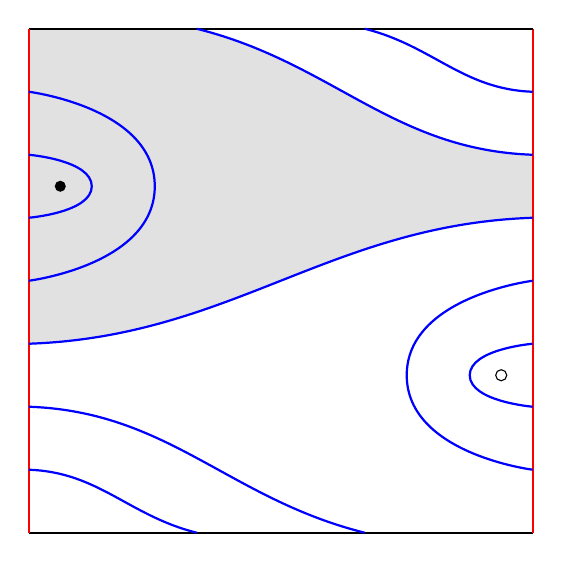
\begin{tikzpicture}[scale = 0.8]
			\draw[thick, black] (0,0) -- (8, 0);
			\draw[thick, red] (8, 0) -- (8, 8);
			\draw[thick, black, name path = B] (8, 8) -- (0, 8);
			\draw[thick, red] (0, 8) -- (0, 0);
			
			\draw[blue, thick] plot[smooth, tension=1.5]
			coordinates {(0,7) (2,5.5) (0,4)};
			\draw[blue, thick] plot[smooth, tension=1.5]
			coordinates {(0,6) (1,5.5) (0,5)};
			
			\draw[blue, thick] plot[smooth, tension=1.5]
			coordinates {(8,4) (6,2.5) (8,1)};
			\draw[blue, thick] plot[smooth, tension=1.5]
			coordinates {(8,3) (7,2.5) (8,2)};
			
			\draw[blue, thick, name path = T2] (0,3) to[out=2, in=-178] (8,5);
			
			\draw[blue, thick] (0,2) to[out=-2, in=166] (5.33333,0);
			\draw[blue, thick] (8,7) to[out=178, in=-14] (5.33333,8);
			\draw[blue, thick] (0,1) to[out=-2, in=166] (2.66667,0);
			\draw[blue, thick, name path = T3] (8,6) to[out=178, in=-14] (2.66667,8);
			
			\fill[black] (0.5,5.5) circle (2.5pt);
			\draw[black] (7.5,2.5) circle (2.5pt);
			\begin{scope}[on background layer]
				\tikzfillbetween[of=T2 and B] {gray!30, opacity=0.8};
				\tikzfillbetween[of=T3 and B] {white!6};
			\end{scope}
		\end{tikzpicture}
	}
\newsavebox{\mypicboxfour}
	\savebox{\mypicboxfour}{
		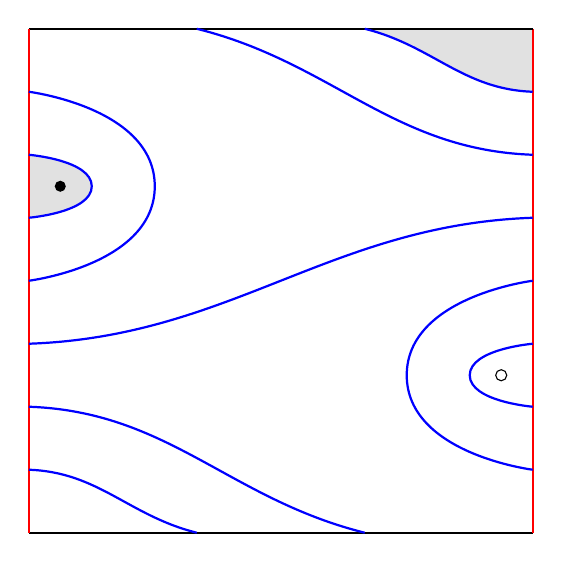
\begin{tikzpicture}[scale=0.8]
			\draw[thick, black] (0,0) -- (8, 0);
			\draw[thick, red] (8, 0) -- (8, 8);
			\draw[thick, black, name path = B] (8, 8) -- (0, 8);
			\draw[thick, red, name path = L] (0, 8) -- (0, 0);
			
			\draw[blue, thick] plot[smooth, tension=1.5]
			coordinates {(0,7) (2,5.5) (0,4)};
			\draw[blue, thick, name path = D] plot[smooth, tension=1.5]
			coordinates {(0,6) (1,5.5) (0,5)};
			
			\draw[blue, thick] plot[smooth, tension=1.5]
			coordinates {(8,4) (6,2.5) (8,1)};
			\draw[blue, thick] plot[smooth, tension=1.5]
			coordinates {(8,3) (7,2.5) (8,2)};
			
			\draw[blue, thick] (0,3) to[out=2, in=-178] (8,5);
			
			\draw[blue, thick] (0,2) to[out=-2, in=166] (5.33333,0);
			\draw[blue, thick, name path = T] (8,7) to[out=178, in=-14] (5.33333,8);
			\draw[blue, thick] (0,1) to[out=-2, in=166] (2.66667,0);
			\draw[blue, thick] (8,6) to[out=178, in=-14] (2.66667,8);
			
			\fill[black] (0.5,5.5) circle (2.5pt);
			\draw[black] (7.5,2.5) circle (2.5pt);
			\begin{scope}[on background layer]
				\tikzfillbetween[of=T and B] {gray!30, opacity=0.8};
				\tikzfillbetween[of=D and L] {gray!30, opacity=0.8};
			\end{scope}
		\end{tikzpicture}
	}
	\begin{figure}[H]
		\centering
			\begin{tikzpicture}
				\node[anchor=south west] at (0,0) {\usebox{\mypicboxthree}};
				\node[anchor=south west] at (6.4,0) {\usebox{\mypicboxfour}};
				\node[anchor=south west] at (0,6.4) {\usebox{\mypicboxone}};
				\node[anchor=south west] at (6.4,6.4) {\usebox{\mypicboxtwo}};
			\end{tikzpicture}
		\caption{The final two disks in the 4-tuple diagram $(7, 2, 1, 3)$.}
	\end{figure}
Throughout, we track the multiplicities of the basepoints $z \text{ and } w$ in these regions, resulting in a list of disks stored in the form $\{(u, v), n_z, n_w, s\}$ where $u, v$ are the intersection points of the disk's gap, and $n_z, n_w$ are the multiplicities of the respective basepoints in the disk. Note that $s$ records which side of the fundamental region the gap is on; for disks with their gap on the left, $s =1$, and for gaps on the right, $s =-1$.

\subsection{Constructing $\text{CFK}^{\infty}$}
Earlier, we defined the $\mathbb{F}[U, U^{-1}]$ module $\text{CFK}^{\infty}(K)$ to be a doubly filtered chain complex, equipped with a boundary operator $\partial$. $\text{CFK}^{\infty}$ can be defined over a field $\mathbb{F}_{pr}$, where $pr$ is any prime, or $\mathbb{Q}$. We will define it over $\mathbb{F}_2$ for the sake of simplicity, meaning all arithmetic is done $\mod{2}$. The $p$ intersection points generate the $\mathbb{F}[U, U^{-1}]$ module. Next, we compute the \textit{Alexander filtration} and \textit{Maslov grading} of the generators using the equations:
\begin{enumerate}[nosep]
	\item $A(u) - A(v) = s \cdot (n_w - n_z)$
	\item $M(u) - M(v) = s \cdot (1 - 2n_w)$
\end{enumerate}
where each disk relates the intersection points (generators) at its endpoints. We solve the two resulting systems of linear equations to get the filtrations and gradings of the generators. Next, we construct the differential. For each disk $d$, we add a term to $\partial$ as follows: record the value of $n_w$ as an exponent on the formal variable $U$. If $s_d = 1$, then we add a $U^{n_w(d)}v_d$ term to $\partial(u_d)$, and if $s_d = -1$, we add a $-U^{n_w(d)}u_d$ term to $\partial(v_d)$. Since we are working over $\mathbb{F}_2$, we note that $-u_d \equiv u_d$, and so we can drop the signs. We also note that  $\partial$ is an $\mathbb{F}[U, U^{-1}]$ module homomorphism, so $\partial(x+y) = \partial(x) +\partial(y)$, and $\partial(U^kx) =U^k\partial(x)$ (equivariant with respect to $U$). The $U$ action respects both filtrations and grading, as we have
\begin{enumerate}[nosep]
	\item $A(Ux) = A(x) - 1$
	\item $i(Ux) = i(x) - 1$
	\item $M(Ux) = M(x) - 2$
\end{enumerate}
for a generator $x$. This leads to a nice graphical representation of $\text{CFK}^{\infty}$ which reveals the meaning behind the $\infty$ superscript and captures the full information of the differential and dual filtrations: we begin by plotting each generator $x$ in $\mathbb{R}^2$ at $(0, A(x))$. We now translate these generators along the diagonal infinitely through action by $U$ and $U^{-1}$, plotting the point $U^kx$ at $(-k, A(x) - k)$, where the first coordinate is the $i$ filtration, and the second coordinate is the Alexander filtration. Finally, we add the arrows between the terms in the differential. We add a vertical arrow if the disk corresponding to it has $n_z \ne 0$, a horizontal arrow if $n_w \ne 0$, and a diagonal arrow if $n_w, \, n_z \ne 0$, where the length corresponds to the basepoint multiplicity. Note that the arrows respect the filtration and grading, so that they can only point down or to the left (or both).
	\begin{figure}[htbp]
		\centering
			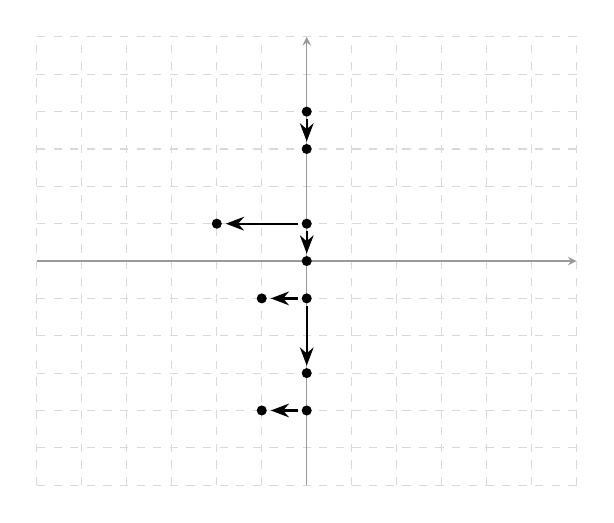
\begin{tikzpicture}
				\begin{axis}[
					axis lines = middle, gray!80,
					xmin=-6, xmax=6,
					ymin=-6, ymax=6,
					grid = both,
					grid style = {dashed, gray!30},
					xticklabel=\empty,
					yticklabel=\empty,
					major tick style = {transparent},
					xtick distance = 1,
					ytick distance = 1
				]
				\addplot[only marks, mark=*, black, mark size=1.6] coordinates {
					(0, 1)
					(0, 4)
					(0, 3)
					(0, 0)
					(0, -1)
					(0, -3)
					(0, -4)
					(-2, 1)
					(-1, -1)
					(-1, -4)
					};
					\addplot[->, -{Stealth}, black, thick] coordinates {(0,3.8) (0,3.2)};
					\addplot[->, -{Stealth}, black, thick] coordinates {(0,0.8) (0,0.2)};
					\addplot[->, -{Stealth}, black, thick] coordinates	{(0,-1.2) (0,-2.8)};
					\addplot[->, -{Stealth}, black, thick] coordinates {(-0.2,1) (-1.8,1)};
					\addplot[->, -{Stealth}, black, thick] coordinates {(-0.2,-4) (-0.8,-4)};
					\addplot[->, -{Stealth}, black, thick] coordinates {(-0.2,-1) (-0.8,-1)};
				\end{axis}
			\end{tikzpicture}
		\caption{The $p$ generators in $(7, 2, 1, 3)$ plotted on the $y$-axis, and the arrows representing $\partial$.}
		\label{fig:fig15}
	\end{figure}
\begin{figure}[H]
	\centering
		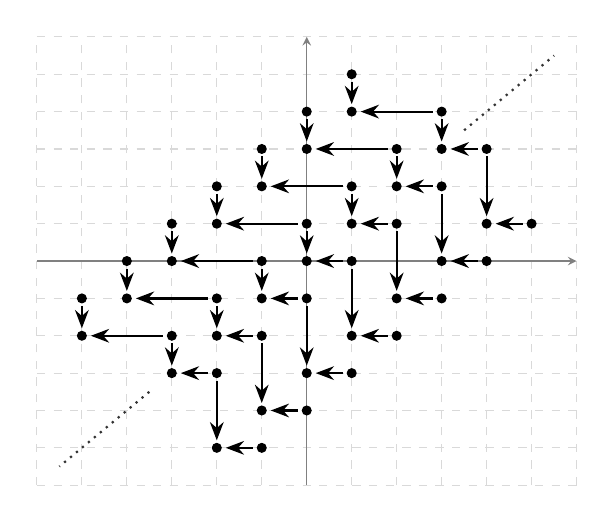
\begin{tikzpicture}
			\begin{axis}[
				axis lines = middle, gray,
				xmin=-6, xmax=6,
				ymin=-6, ymax=6,
				grid = both,
				grid style = {dashed, gray!30},
				xticklabel=\empty,
				yticklabel=\empty,
				major tick style = {transparent},
				xtick distance = 1,
				ytick distance = 1
			]
			\foreach \t in {-1, 0, 1, 2, 3, 4, 5}{
				\addplot[only marks, mark=*, black, mark size=1.6] coordinates {
				 (\t, \t-4)
				(\t-1, \t-4)
				(\t-1, \t-2)
				(\t-2, \t-2)
				(\t-2, \t-1)
				(\t-4, \t-1)
				(\t-4, \t)
				};
				\addplot[->, -{Stealth}, black, thick] coordinates {(\t-0.2, \t-4) (\t-0.8, \t-4)};
				\addplot[->, -{Stealth}, black, thick] coordinates {(\t-1, \t-2.2) (\t-1, \t-3.8)};
				\addplot[->, -{Stealth}, black, thick] coordinates {(\t-1.2, \t-2) (\t-1.8, \t-2)};
				\addplot[->, -{Stealth}, black, thick] coordinates {(\t-2, \t-1.2) (\t-2, \t-1.8)};
				\addplot[->, -{Stealth}, black, thick] coordinates {(\t-2.2, \t-1) (\t-3.8, \t-1)};
				\addplot[->, -{Stealth}, black, thick] coordinates {(\t-4, \t-0.2) (\t-4, \t-0.8)};
			}
			\draw[-, thick, dotted, black, opacity = 0.8] (3.5,3.5) -- (5.5,5.5);
			\draw[-, thick, dotted, black, opacity = 0.8] (-3.5,-3.5) -- (-5.5,-5.5);
			\end{axis}
		\end{tikzpicture}
	\caption{The full $\text{CFK}^{\infty}$ complex for the knot parametrized by $(7, 2, 1, 3)$.}
\end{figure}

\subsection{Recap of the Computational Process}
	\begin{enumerate}
		\item Begin with a Heegaard diagram of your knot $K$ in $S^3$.
		\item Move to the fundamental domain of the torus and parametrize the diagram with a 4-tuple $(p, a, b, r)$.
		\item Count all the embedded bigons (disks) in the resulting 4-tuple diagram using the described algorithm.
		\item Construct $\text{CFK}^{\infty}(K)$ from this information.
		\item Finally, we can compute knot invariants like $\tau, \epsilon, \nu, \Upsilon$ using the chain complex and  the associated gradings and filtrations.
	\end{enumerate}

\section{An Example of a Knot Floer Invariant: $\tau$}
\subsection{Knot Concordance}
\textit{Knot concordance} is a central concept in knot theory. Given two knots $K_1$, $K_2$, we say $K_1$ and $K_2$ are \textit{concordant} if there is a smooth embedding of $S^1 \times [0,1]$ into $S^3 \times [0,1]$ whose boundary is the knots $K_1$ and $-K_2$ in $S^3 \times \{0\}$ and $S^3 \times \{1\}$ respectively \cite[Section~1]{livingston2004surveyclassicalknotconcordance}. It is straightforward to see that knot concordance is an equivalence relation. We can now define the \textit{knot concordance group} $\mathcal{C}$, which is the abelian group of all knot types modulo concordance, with the connected sum $\#$ as the group operation. We say a knot is \textit{slice} if it is in the same equivalence class as the unknot. We define also a \textit{slice surface}: given a knot $K \subset S^3$, a slice surface for $K$ is a smooth submanifold-with-boundary $\mathcal{M} \subset B^4$ such that $\partial \mathcal{M} = K$. The \textit{four ball genus} of a knot $g_4(K)$ is the minimal genus of any slice surface for $K$. $g_4(K)$ gives a lower bound on the unknotting number $u(K)$ \cite[Section~1]{Ozsv_th_2003}. We now examine an invariant providing a lower bound on $g_4(K)$.

\subsection{$\tau(K)$}
The interested reader is encouraged to read \cite[Section~1]{Ozsv_th_2003} for a complete and rigorous definition of $\tau(K)$. For our purposes, it is mostly important to know that $\tau(K)$ is an integer valued \textit{concordance invariant}, meaning that for two concordant knots $K_1$ and $K_2$ , we have $\tau(K_1) = \tau(K_2)$. It also induces a homomorphism from the concordance group $\mathcal{C}$ to $\mathbb{Z}$ \cite[Theorem~1.2]{Ozsv_th_2003}, so we have $\tau(K_1 \# K_2) = \tau(K_1) + \tau(K_2)$.  $\tau(K)$ has two key properties: as mentioned, it is a lower bound on $g_4(K)$ and $u(K)$ \cite[Corollary~1.3]{Ozsv_th_2003}, and it obstructs sliceness, meaning that if a knot $K$ is smoothly slice, we have $\tau(K) = 0$. Because concordance is an equivalence relation, for any knot $K$, $K \# mK$ is concordant to the unknot, where $mK$ denotes the mirror of $K$. It follows directly from the above properties that $\tau(K) = -\tau(mK)$.

\subsection{Another Flavour:  $\widehat{\text{CFK}}$}
Up until now, we have only discussed the  $\text{CFK}^{\infty}$ chain complex. It turns out that this structure is overkill in many cases. We can instead work with a simpler chain complex,  $\widehat{\text{CFK}}$. Roughly speaking,  $\widehat{\text{CFK}}(K)$ is obtained from looking at only the generators and arrows that fall on the $y$ axis in the graph of  $\text{CFK}^{\infty}(K)$, i.e. the generators with $i$ filtration $0$. The differential $\partial$ is constructed from the disks with $n_w = 0$. We note that $\mathcal{H}_{*}(\widehat{\text{CFK}}(K)) \cong \mathbb{F}$, i.e. the total homology is always generated by a single nonzero homology class $[x]$ \cite[Section~2]{OzsvathSzabo2017}. Similarly to the $\infty$ flavour, $\widehat{\text{CFK}}(K)$ is an $\mathbb{F}$ module generated by the $p$ intersection points in the Heegaard diagram, equipped with the same Alexander filtrations and Maslov gradings as before. This complex is filtered by the Alexander filtration: when we write $\widehat{\text{CFK}}(K)_{\le s}$, we mean the subcomplex containing all generators with Alexander filtration $\le s$, along with $\partial$ restricted to these generators. Note that $\emptyset = \widehat{\text{CFK}}(K)_{\le i-n} \subset ... \subset \widehat{\text{CFK}}(K)_{\le i} \subset \widehat{\text{CFK}}(K)_{\le i +1} \subset ... \subset  \widehat{\text{CFK}}(K)_{\le i+n}  = \widehat{\text{CFK}}(K)$, i.e. the subcomplexes are eventually empty or the full complex for large enough $n \in \mathbb{Z}$.
	\begin{figure}[H]
		\centering
			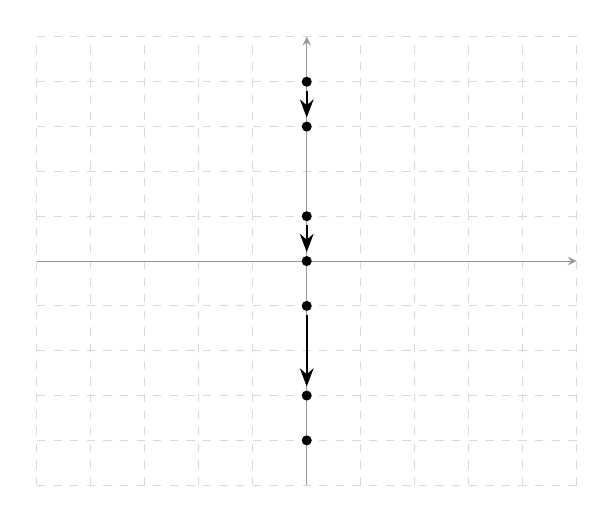
\begin{tikzpicture}
				\begin{axis}[
					axis lines = middle, gray!80,
					xmin=-5, xmax=5,
					ymin=-5, ymax=5,
					grid = both,
					grid style = {dashed, gray!30},
					xticklabel=\empty,
					yticklabel=\empty,
					major tick style = {transparent},
					xtick distance = 1,
					ytick distance = 1
				]
				\addplot[only marks, mark=*, black, mark size=1.6] coordinates {
					(0, 1)
					(0, 4)
					(0, 3)
					(0, 0)
					(0, -1)
					(0, -3)
					(0, -4)
					};
					\addplot[->, -{Stealth}, black, thick] coordinates {(0,3.8) (0,3.2)};
					\addplot[->, -{Stealth}, black, thick] coordinates {(0,0.8) (0,0.2)};
					\addplot[->, -{Stealth}, black, thick] coordinates	{(0,-1.2) (0,-2.8)};
				\end{axis}
			\end{tikzpicture}
		\caption{$\widehat{\text{CFK}}(K)$ of $(7, 2, 1, 3)$.}
		\label{fig:fig17}
	\end{figure}

\subsection{Computing $\tau(K)$ from $\widehat{\text{CFK}}(K)$}
The standard definition of $\tau(K)$ is as follows: first, let $\mathcal{H}_{*}(\widehat{\text{CFK}}(K)_{\le s}, \partial)$ be the homology of the subcomplex of generators with Alexander filtration $\le s$. Note that this is well defined, since $A(\partial(x)) \le A(x)$, and so $ x \in \widehat{\text{CFK}}(K)_{\le s} \implies \partial(x) \in \widehat{\text{CFK}}(K)_{\le s}$. Now, define the map $\iota_s \colon  \mathcal{H}_{*}(\widehat{\text{CFK}}(K)_{\le s}) \to \mathcal{H}_{*}(\widehat{\text{CFK}}(K)) \cong \mathbb{F}$ to be the map induced on homology by the inclusion of the subcomplex $(\widehat{\text{CFK}}(K)_{\le s})$ into $\widehat{\text{CFK}}(K)$. Finally, we define \[\tau(K) \coloneq \min_{s \in \mathbb{Z}} \{ s \mid \iota_s \text{ is non-trivial.} \} \]  \cite[Definition~3.1]{Golla_2015}. While the rigorous definition is somewhat dense, in practice, the computation is straightforward. We continue working with the complex from the 4-tuple diagram $(7, 2, 1, 3)$.
	\begin{figure}[H]\vspace{-0.4cm}
		\centering
			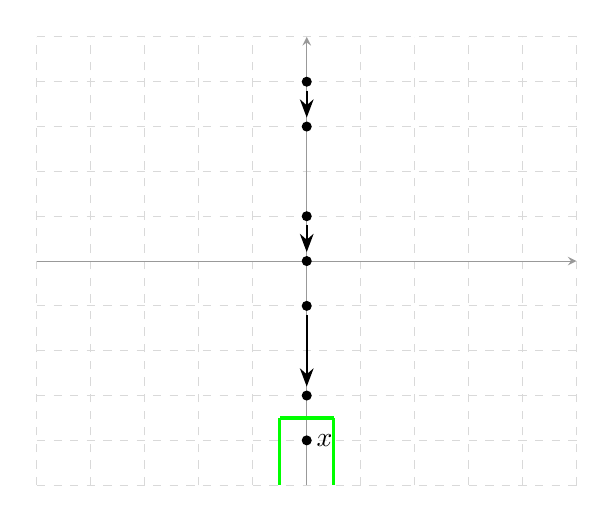
\begin{tikzpicture}
				\begin{axis}[
					axis lines = middle, gray!80,
					xmin=-5, xmax=5,
					ymin=-5, ymax=5,
					grid = both,
					grid style = {dashed, gray!30},
					xticklabel=\empty,
					yticklabel=\empty,
					major tick style = {transparent},
					xtick distance = 1,
					ytick distance = 1
				]
				\addplot[only marks, mark=*, black, mark size=1.6] coordinates {
					(0, 1)
					(0, 4)
					(0, 3)
					(0, 0)
					(0, -1)
					(0, -3)
					(0, -4)
					};
					\addplot[->, -{Stealth}, black, thick] coordinates {(0,3.8) (0,3.2)};
					\addplot[->, -{Stealth}, black, thick] coordinates {(0,0.8) (0,0.2)};
					\addplot[->, -{Stealth}, black, thick] coordinates	{(0,-1.2) (0,-2.8)};
					\addplot[-, green, very thick] coordinates {(0.5,-3.5) (-0.5,-3.5)};
					\addplot[-, green, very thick] coordinates {(0.5,-3.5) (0.5,-5)};
					\addplot[-, green, very thick] coordinates {(-0.5,-3.5) (-0.5,-5)};
					\node[anchor=west, black] at (axis cs:0, -4) {$x$};
				\end{axis}
			\end{tikzpicture}
		\caption{$\widehat{\text{CFK}}(K)_{\le -4}$ of $(7, 2, 1, 3)$  boxed in green.}
		\label{fig:fig18}
	\end{figure}\vspace{-0.3cm}
Let us first compute the total homology $\mathcal{H}_{*}(\widehat{\text{CFK}}(K))$. By inspection, we note that the only generator in $\ker(\partial)$ that isn't in $\operatorname{im}(\partial)$ is $x$. Hence, $\mathcal{H}_{*}(\widehat{\text{CFK}}(K)) \cong \mathbb{F}\langle x \rangle$. Notice that the generator $x$ survives homology of the subcomplex $\widehat{\text{CFK}}(K)_{\le -4}$, so $\mathcal{H}_{*}(\widehat{\text{CFK}}(K)_{\le -4}) \cong \mathbb{F}\langle x \rangle$. Thus, the induced map $\iota_{-4} \colon  \mathcal{H}_{*}(\widehat{\text{CFK}}(K)_{\le -4}) \to \mathcal{H}_{*}(\widehat{\text{CFK}}(K)) \cong \mathbb{F}$ is non trivial (it is the identity map, and the homology class of $x$ is nonzero). Now, observe that for $s \le -5$, the subcomplex $\widehat{\text{CFK}}(K)_{\le s}$ is empty, and hence the map $\iota_s$ is trivial. We find that $\tau((7, 2, 1, 3)) = -4$. \\
\\
Let us look at another example: consider the 4-tuple diagram $(3, 1, 1, 2)$, which parametrizes the righthanded trefoil.
	\begin{figure}[H]
		\centering
			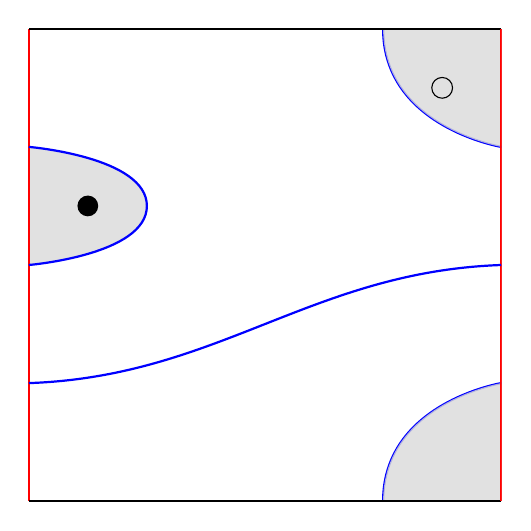
\begin{tikzpicture}[scale=1.5]
				\draw[thick, black] (0,0) -- (4, 0);
				\draw[thick, red, name path = R] (4, 0) -- (4, 4);
				\draw[thick, black] (4, 4) -- (0, 4);
				\draw[thick, red, name path = L] (0, 4) -- (0, 0);
				
				\draw[blue, thick, name path = Ld] plot[smooth, tension=1.5]
				coordinates {(0,3) (1,2.5) (0,2)};
				
				\begin{scope}
				\clip (0,0) rectangle (4,4);
				\draw[blue, thick, name path = Rd1] plot[smooth, tension=1.5]
				coordinates {(4,1) (3,0) (4,-1)};
				\tikzfillbetween[of=R and Rd1] {gray!30, opacity=0.8};
				\draw[thick, black] (0,0) -- (4, 0);
				\draw[thick, red] (4, 0) -- (4, 4);
				\end{scope}
				
				\begin{scope}
				\clip (0,0) rectangle (4,4);
				\draw[blue, thick, name path = Rd2] plot[smooth, tension=1.5]
				coordinates {(4,3) (3,4) (4,5)};
				\tikzfillbetween[of=R and Rd2] {gray!30, opacity=0.8};
				\draw[thick, black] (4, 4) -- (0, 4);
				\draw[thick, red] (4, 0) -- (4, 4);
				\end{scope}
				
				\draw[blue, thick] (0,1) to[out=2, in=-178] (4,2);
				
				\fill[black] (0.5,2.5) circle (2.5pt);
				\draw[black] (3.5,3.5) circle (2.5pt);
				\begin{scope}[on background layer]
					\tikzfillbetween[of=L and Ld] {gray!30, opacity=0.8};
				\end{scope}
			\end{tikzpicture}
			\hspace{1cm}
			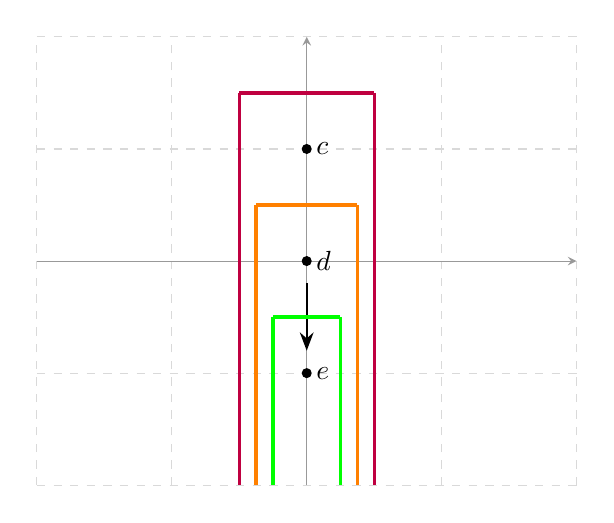
\begin{tikzpicture}[scale=1]
				\begin{axis}[
					axis lines = middle, gray!80,
					xmin=-2, xmax=2,
					ymin=-2, ymax=2,
					grid = both,
					grid style = {dashed, gray!30},
					xticklabel=\empty,
					yticklabel=\empty,
					major tick style = {transparent},
					xtick distance = 1,
					ytick distance = 1
				]
				\addplot[only marks, mark=*, black, mark size=1.6] coordinates {
					(0, 1)
					(0, 0)
					(0, -1)
					};
					\addplot[->, -{Stealth}, black, thick] coordinates {(0,-0.2) (0,-0.8)};
					\node[anchor=west, black] at (axis cs:0, 1) {$c$};
					\node[anchor=west, black] at (axis cs:0, 0) {$d$};
					\node[anchor=west, black] at (axis cs:0, -1) {$e$};
					\addplot[-, green, very thick] coordinates {(0.25,-0.5) (-0.25,-0.5)};
					\addplot[-, green, very thick] coordinates {(0.25,-0.5) (0.25,-2)};
					\addplot[-, green, very thick] coordinates {(-0.25,-0.5) (-0.25,-2)};
					\addplot[-, orange, very thick] coordinates {(0.375,0.5) (-0.375,0.5)};
					\addplot[-, orange, very thick] coordinates {(0.375,0.5) (0.375,-2)};
					\addplot[-, orange, very thick] coordinates {(-0.375,0.5) (-0.375,-2)};
					\addplot[-, purple, very thick] coordinates {(0.5,1.5) (-0.5,1.5)};
					\addplot[-, purple, very thick] coordinates {(0.5,1.5) (0.5,-2)};
					\addplot[-, purple, very thick] coordinates {(-0.5,1.5) (-0.5,-2)};
				\end{axis}
			\end{tikzpicture}
		\caption{The 4-tuple diagram $(3, 1, 1, 2)$ with the two disks shaded in grey; $\widehat{\text{CFK}}(K)$ of $(3, 1, 1, 2)$ along with the three relevant subcomplexes.}
		\label{fig:fig19} 
	\end{figure}
If we look at the total homology  $\mathcal{H}_{*}(\widehat{\text{CFK}}(K)) \coloneq \ker(\partial) / \operatorname{im} = \langle c, e \rangle / \langle e \rangle$, we can see that the nonzero homology class is $[c]$, and so $\mathcal{H}_{*}(\widehat{\text{CFK}}(K)) \cong \mathbb{F} \langle c \rangle$. We compute the homology of the subcomplexes $\mathcal{H}_{*}(\widehat{\text{CFK}}(K)_{\le -1}) \cong \mathbb{F} \langle e \rangle$ and $\mathcal{H}_{*}(\widehat{\text{CFK}}(K)_{\le 0}) = \langle e \rangle / \langle  e \rangle = 0$. Hence, $\iota_{-1}$ is trivial (the homology class $[e]$ maps to $0$ in the total homology) and $\iota_0$ is trivial as $\mathcal{H}_{*}(\widehat{\text{CFK}}(K)_{\le 0})$ is trivial. For $s \le -2$, once again the subcomplex is empty. Looking at $\widehat{\text{CFK}}(K)_{\le 1}$, we notice that $\widehat{\text{CFK}}(K)_{\le 1} = \widehat{\text{CFK}}(K)$, and so the map $\iota_1$ is the identity, sending $[c]$ to $[c]$. Hence, $\tau((3, 1, 1, 2)) = 1$.

\subsection{An Open Question}
Throughout, we have defined both $\text{CFK}^{\infty}$ and $\widehat{\text{CFK}}$ over $\mathbb{F}_2$ for simplicity. Recall that we can define these complexes over any prime field $\mathbb{F}_p$, or over the rationals $\mathbb{Q}$. Being specific with notation, let $\tau_{\mathbb{F}}(K)$ be the above invariant along with the field it is calculated over. The question is whether our choice of $\mathbb{F}$ affects the value of $\tau_{\mathbb{F}}(K)$. More formally, does there exist some knot $K$ along with two fields $\mathbb{F}, \mathbb{F}^{'}$ such that $\tau_{\mathbb{F}}(K) \ne \tau_{\mathbb{F}^{'}}(K)$? This question remains unanswered as of today.

\section{Goals and Results}

\subsection{Goals}
The main goal of this project was to implement the above algorithm to compute $\text{CFK}^{\infty}$ for any $(1,1)$-knot, then to compute as many invariants as possible from this information. Though many software packages can compute the knot Floer homology of an arbitrary knot, they fail to capture the full information of $\text{CFK}^{\infty}$, as they throw away any diagonal arrows in the complex. In the $(1,1)$ context, this is not necessary, as we can construct the full complex directly from the 4-tuple diagram. Hence, this algorithm is an improvement over previous implementations and enables the computation of more complex invariants, such as the concordance invariant $\Upsilon_K(t)$, defined by Ozsv\'ath, Szab\'o and Stipsicz \cite[Section~1.1]{Ozsv_th_2017} , which assigns a continuous, piecewise linear function to a knot.

\begin{figure}[htbp!]
	\centering
		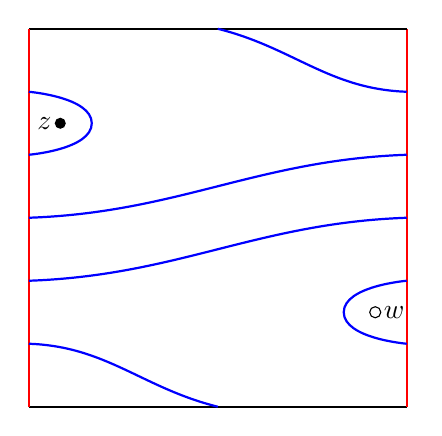
\begin{tikzpicture}[scale=0.8]
		\draw[thick, black] (0,0) -- (6, 0);
		\draw[thick, red] (6, 0) -- (6, 6);
		\draw[thick, black] (6, 6) -- (0, 6);
		\draw[thick, red] (0, 6) -- (0, 0);
		
		\draw[blue, thick] plot[smooth, tension=1.5]
		coordinates {(0,5) (1,4.5) (0,4)};
		
		\draw[blue, thick] plot[smooth, tension=1.5]
		coordinates {(6,2) (5,1.5) (6,1)};
		
		\draw[blue, thick] (0,3) to[out=2, in=-178] (6,4);
		\draw[blue, thick] (0,2) to[out=2, in=-178] (6,3);
		
		\draw[blue, thick] (0,1) to[out=-2, in=166] (3,0);
		\draw[blue, thick] (6,5) to[out=178, in=-14] (3,6);
		
		\fill[black] (0.5,4.5) circle (2.5pt);
		\draw[black] (5.5,1.5) circle (2.5pt);
		\node at (0.25, 4.5) {$z$};
		\node at (5.8, 1.5) {$w$};
		\end{tikzpicture}
		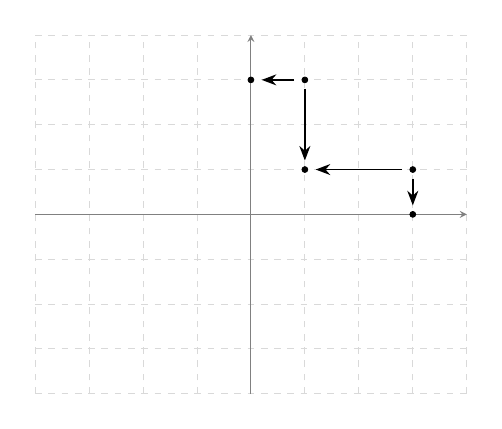
\begin{tikzpicture}[scale=0.8]
			\begin{axis}[
				axis lines = middle, gray,
				xmin=-4, xmax=4,
				ymin=-4, ymax=4,
				grid = both,
				grid style = {dashed, gray!30},
				xticklabel=\empty,
				yticklabel=\empty,
				major tick style = {transparent},
				xtick distance = 1,
				ytick distance = 1
				]
				\addplot[only marks, mark=*, black, mark size=1.3] coordinates {
				(0,3)
				(1,3)
				(1,1)
				(3,1)
				(3,0)
				};
				\addplot[->, -{Stealth}, black, thick] coordinates {(0.8, 3) (0.2, 3)};
				\addplot[->, -{Stealth}, black, thick] coordinates {(1, 2.8) (1, 1.2)};
				\addplot[->, -{Stealth}, black, thick] coordinates {(2.8, 1) (1.2, 1)};
				\addplot[->, -{Stealth}, black, thick] coordinates {(3, 0.8) (3, 0.2)};
			\end{axis}
		\end{tikzpicture}
		\begin{tikzpicture}[scale=0.8]
			\begin{axis}[
				axis lines = middle, gray,
				xmin=-0.75, xmax=2.75,
				ymin=-2.75, ymax=0.75,
   				xlabel = $t$, ylabel = $\Upsilon_{T_{3,4}}(t)$,
				label style = {black},
				grid = both,
				grid style = {dashed, gray!30},
				xtick distance = 1,
				ytick distance = 1
				]
				\addplot[black, thick, domain = 0:2/3]  {-3*x};
				\addplot[black, thick, domain = 2/3:4/3]  {-2};
				\addplot[black, thick, domain = 4/3:2]  {-6+3*x};
				\addplot[only marks, mark=*, black, mark size=1.3] coordinates {
				(0,0)
				(2,0)
				(2/3,-2)
				(4/3,-2)
				};
			\end{axis}
		\end{tikzpicture}
	\caption{From left to right: the 4-tuple diagram $(5, 1, 2, 2)$, which parametrizes the knot $T_{3,4}$; part of the complex $\text{CFK}^{\infty}(T_{3,4})$; and $\Upsilon_{T_{3,4}}(t)$.}
	\label{fig:fig20}
\end{figure}

\subsection{Significance of  $\Upsilon_K(t)$}
As mentioned above, the information of the full complex allows us to compute $\Upsilon_K(t)$, though the implementation is somewhat non-trivial. In fact, this program is the first apppearance of a software which can compute $\Upsilon_K(t)$ on such a broad family of knots. Previously, such algorithms existed only for simpler families like the torus knots or Floer-thin knots. The interested reader is greatly encouraged to read \cite{Ozsv_th_2017} for a full treatment of this invariant: we quickly note here that it is a strict improvement over $\tau(K)$, as we have $\Upsilon_K(t) = -\tau(k) \cdot t$ for small enough $t$. Note that if $K$ is concordant to the unknot, then $\Upsilon_K(t) \equiv 0$. It becomes clear that we can have two knots $K_1, K_2$ such that $\tau(K_1 \# K_2) = 0$, but  $\Upsilon_{K_1 \# K_2}(t) \not\equiv 0$. 

This is illustrated in the following example: let $K_1 = T_{3,4}, K_2 = T_{2,-7}$. Note that $K_1$ and $K_2$ are parametrized by $(5, 1, 2, 2)$ and $(7, 1, 5, 1)$ respectively. Then, using the standard formula $\tau(T_{p, q}) =\frac{(p - 1)(q - 1)}{2}$  \cite[Theorem~4.7]{OzsvathSzabo2017}, we find that $\tau(K_1) = 3$ and $\tau(K_2) = -3$. Clearly, $\tau(K_1 \# K_2) = 0$. Now, we compute $\Upsilon_{K_1}(t)$ and $\Upsilon_{K_2}(t)$, using \cite[Corollary~2.3]{Feller_2017}, and \cite[Example~1.16]{Ozsv_th_2017}. We note that $T_{2, -7}$ is the mirror of $T_{2, 7} = T_{2, 3 \cdot 2+1}$, and as such $\Upsilon_{K_2}(t) = -\Upsilon_{T_{2, 7}}(t)$ \cite[Proposition~1.9]{Ozsv_th_2017}. Using all of these facts, we obtain
\[ 
\Upsilon_{K_1}(t) = 
	\begin{cases}
		-3t, & 0 \le t \le 2/3,\\[1mm]
		-2, & 2/3 \le t \le 4/3, \\[1mm]
		-6+3t, & 4/3 \le t \le 2.
	\end{cases}
\]
and
\[ 
\Upsilon_{K_2}(t) = 
	\begin{cases}
		3t, & 0 \le t \le 1,\\[1mm]
		6-3t, & 1 \le t \le 2.
	\end{cases}
\]
\begin{figure}[H]
		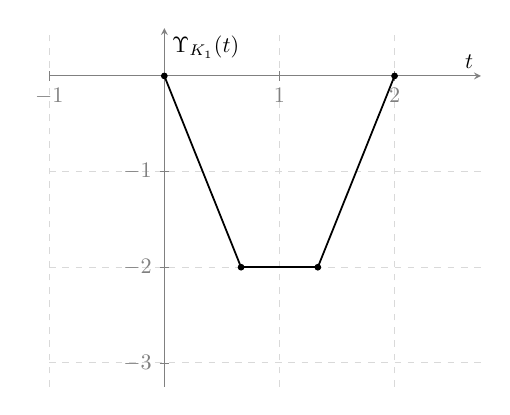
\begin{tikzpicture}[scale=0.8]
			\begin{axis}[
				axis lines = middle, gray,
				xmin=-1, xmax=2.75,
				ymin=-3.25, ymax=0.5,
   				xlabel = $t$, ylabel = $\Upsilon_{K_1}(t)$,
				label style = {black},
				grid = both,
				grid style = {dashed, gray!30},
				xtick distance = 1,
				ytick distance = 1
				]
				\addplot[black, thick, domain = 0:2/3]  {-3*x};
				\addplot[black, thick, domain = 2/3:4/3]  {-2};
				\addplot[black, thick, domain = 4/3:2]  {-6+3*x};
				\addplot[only marks, mark=*, black, mark size=1.3] coordinates {
				(0,0)
				(2,0)
				(2/3,-2)
				(4/3,-2)
				};
			\end{axis}
		\end{tikzpicture}
		\hspace{1cm}
		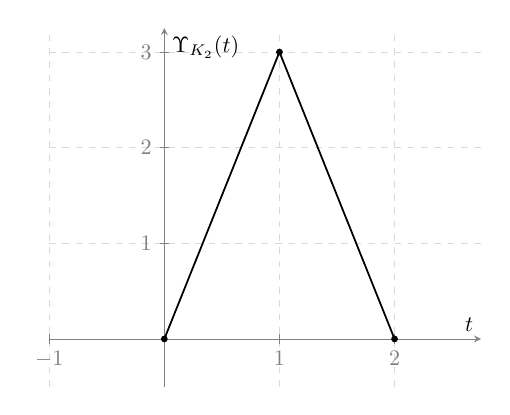
\begin{tikzpicture}[scale=0.8]
			\begin{axis}[
				axis lines = middle, gray,
				xmin=-1, xmax=2.75,
				ymin=-0.5, ymax=3.25,
   				xlabel = $t$, ylabel = $\Upsilon_{K_2}(t)$,
				label style = {black},
				grid = both,
				grid style = {dashed, gray!30},
				xtick distance = 1,
				ytick distance = 1
				]
				\addplot[black, thick, domain = 0:1]  {3*x};
				\addplot[black, thick, domain = 1:2]  {6-3*x};
				\addplot[only marks, mark=*, black, mark size=1.3] coordinates {
				(0,0)
				(2,0)
				(1, 3)
				};
			\end{axis}
		\end{tikzpicture}
	\caption{$\Upsilon_{K_1}(t)$ and $\Upsilon_{K_2}(t)$.}
	\label{fig:fig21}
\end{figure}
It is immediately obvious that $\Upsilon_{K_1 \# K_2} = \Upsilon_{K_1}(t) + \Upsilon_{K_2}(t) \not\equiv 0$. Hence, $\Upsilon_{K_1 \# K_2}(t)$ tells us that $K_1 \# K_2$ is not concordant to the unknot where $\tau(K_1 \# K_2)$ is not strong enough to do so.
\begin{figure}[H]
		\begin{tikzpicture}[scale=0.8]
			\begin{axis}[
				axis lines = middle, gray,
				xmin=-1, xmax=2.75,
				ymin=-0.5, ymax=3.25,
   				xlabel = $t$, ylabel = $\Upsilon_{K_1 \# K_2}(t)$,
				label style = {black},
				grid = both,
				grid style = {dashed, gray!30},
				xtick distance = 1,
				ytick distance = 1
				]
				\addplot[black, thick, domain = 0:2/3]  {0};
				\addplot[black, thick, domain = 2/3:1]  {3*x-2};
				\addplot[black, thick, domain = 1:4/3]  {4-3*x};
				\addplot[black, thick, domain = 4/3:2]  {0};
				\addplot[only marks, mark=*, black, mark size=1.3] coordinates {
				(0,0)
				(2,0)
				(2/3,0)
				(1,1)
				(4/3,0)
				};
			\end{axis}
		\end{tikzpicture}
	\caption{$\Upsilon_{K_1 \# K_2}(t)$.}
	\label{fig:fig22}
\end{figure}

\subsection{Results}
The $(1,1)$ family gives us an infinite and convenient search space, as we can simply iterate over all valid 4-tuples and check if they parametrize a knot. We have leveraged this fact, and the program implementing the algorithm and invariants described above, to compute $\text{CFK}^{\infty}(K), \epsilon(K), \nu(K), g(K), \tau(K), \text{ and } \Upsilon_K(t)$ for all knots parametrized by 4-tuples $(p, a, b, r)$ with $p \le 129$. Additionally, we have investigated the open question regarding $\tau_{\mathbb{F}_{pr}}(K)$, confirming that there are no knots parametrized by 4-tuples with $p \le 145$ such that $\tau_{\mathbb{F}_{pr}}(K)$ differs for any $pr \in \{2, 3, 5, 7, 11, 13\}$.

From here, we hope to implement a computation for $\tau_{\mathbb{Q}}(K)$, in order to investigate potential phenomena in another context. We are also looking into infinite families of mutually non concordant knots by finding families of 4-tuples parametrizing knots $\{K_n\}_{n=0}^{\infty}$ such that any knot $K$ which is a linear combination of knots in this family has $\Upsilon_K(t) \not\equiv 0$. $\text{CFK}^{\infty}$ of a knot from such a family is pictured below.

\begin{figure}[H]
		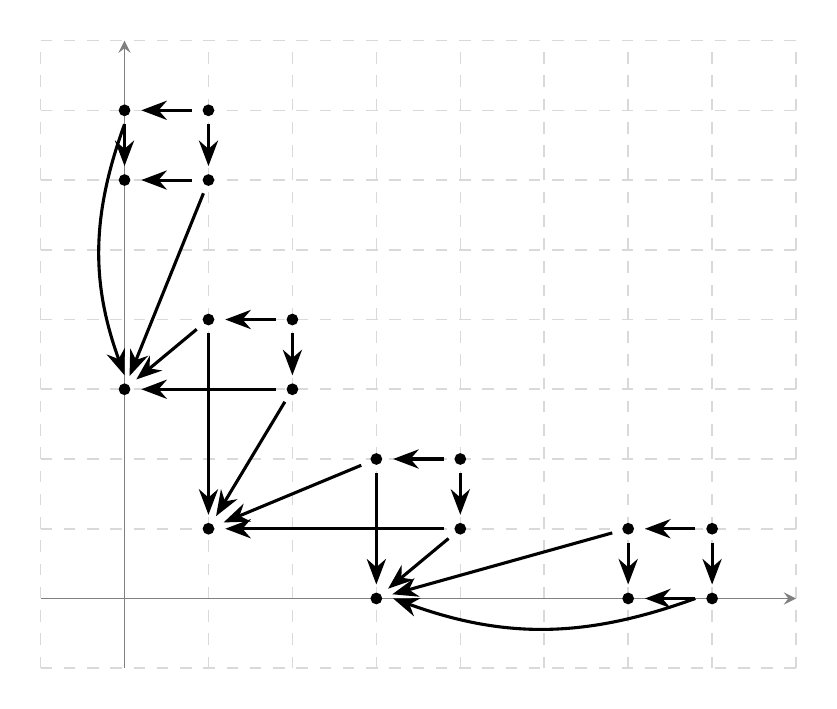
\begin{tikzpicture}[scale=1.4]
			\begin{axis}[
			axis lines = middle, gray,
			xmin=-1, xmax=8,
			ymin=-1, ymax=8,
			grid = both,
			grid style = {dashed, gray!30},
			xticklabel=\empty,
			yticklabel=\empty,
			major tick style = {transparent},
			xtick distance = 1,
			ytick distance = 1
			]
			\addplot[only marks, mark=*, black, mark size=1.3] coordinates {
			(6, 1)
			(7, 1)
			(7, 0)
			(6, 0)
			(3, 0)
			(1, 1)
			(0, 3)
			(0, 6)
			(0, 7)
			(1, 7)
			(1, 6)
			(1, 4)
			(2, 4)
			(2, 3)
			(3, 2)
			(4, 2)
			(4, 1)
			};
			\addplot[->, -{Stealth}, black, thick] coordinates {(6, 0.8) (6, 0.2)};
			\addplot[->, -{Stealth}, black, thick] coordinates {(5.81, 0.94) (3.19, 0.06)};
			\addplot[->, -{Stealth}, black, thick] coordinates {(7, 0.8) (7, 0.2)};
			\addplot[->, -{Stealth}, black, thick] coordinates {(6.8, 1) (6.2, 1)};
			\draw[->, -{Stealth}, black, thick, bend left =20] (6.8, 0) to (3.2, 0);
			\addplot[->, -{Stealth}, black, thick] coordinates {(6.8, 0) (6.2, 0)};
			\draw[->, -{Stealth}, black, thick, bend right = 20] (0, 6.8) to (0, 3.2);
			\addplot[->, -{Stealth}, black, thick] coordinates {(0, 6.8) (0, 6.2)};
			\addplot[->, -{Stealth}, black, thick] coordinates {(0.8, 7) (0.2, 7)};
			\addplot[->, -{Stealth}, black, thick] coordinates {(1, 6.8) (1, 6.2)};
			\addplot[->, -{Stealth}, black, thick] coordinates {(0.8, 6) (0.2, 6)};
			\addplot[->, -{Stealth}, black, thick] coordinates {(0.94, 5.81) (0.06, 3.19)};
			\addplot[->, -{Stealth}, black, thick] coordinates {(1, 3.8) (1, 1.2)};
			\addplot[->, -{Stealth}, black, thick] coordinates {(0.86, 3.86) (0.14, 3.14)};
			\addplot[->, -{Stealth}, black, thick] coordinates {(1.8, 4) (1.2, 4)};
			\addplot[->, -{Stealth}, black, thick] coordinates {(2, 3.8) (2, 3.2)};
			\addplot[->, -{Stealth}, black, thick] coordinates {(1.8, 3) (0.2, 3)};
			\addplot[->, -{Stealth}, black, thick] coordinates {(1.91, 2.82) (1.09, 1.18)};
			\addplot[->, -{Stealth}, black, thick] coordinates {(3, 1.8) (3, 0.2)};
			\addplot[->, -{Stealth}, black, thick] coordinates {(2.82, 1.91) (1.18, 1.09)};
			\addplot[->, -{Stealth}, black, thick] coordinates {(4, 1.8) (4, 1.2)};
			\addplot[->, -{Stealth}, black, thick] coordinates {(3.8, 2) (3.2, 2)};
			\addplot[->, -{Stealth}, black, thick] coordinates {(3.8, 1) (1.2, 1)};
			\addplot[->, -{Stealth}, black, thick] coordinates {(3.86, 0.86) (3.14, 0.14)};
			\end{axis}
		\end{tikzpicture}
	\caption{Part of $\text{CFK}^{\infty}((17, 2, 4, 4)).$}
\end{figure}

\nocite{*}
\bibliographystyle{amsalpha}
\bibliography{bibliography}

\end{document}


